\newpage
\subsection{Goal}

The useage of direct methods (one-dimensional methods of exhaustive search, dichotomy, golden section search; multidimensional methods of exhaustive search, Gauss, Nelder-Mead) in the tasks of unconstrained nonlinear optimization.

\subsection{Formulation of the problem}

\paragraph{I.}

Use the one-dimensional methods of \textit{exhaustive search}, \textit{dichotomy} and \textit{golden section} search to find an approximate (with precision $\varepsilon = 0.001$) solution $x: f(x) \rightarrow \min$  for the following functions and domains:

\begin{enumerate}
    \item $f(x) = x^3, x \in [0, 1]$;
    \item $f(x) = \lvert x - 0.2 \rvert, x \in [0, 1]$;
    \item $f(x) = x\sin{\frac{1}{x}}, x \in [0.01, 1]$.
\end{enumerate}

Calculate the number of $f$-calculations and the number of iterations performed in each method and analyze the results.
Explain differences (if any) in the results obtained.

\paragraph{II.}

Generate random numbers $\alpha \in (0, 1)$ and $\beta \in (0, 1)$.
Furthermore, generate the noisy data $\{x_k, y_k\}$, where $k = 0, ..., 100$, according to the following rule:

\begin{equation}
    y_k = \alpha x_k + \beta + \delta_k, x_k = \frac{k}{100},
\end{equation}

where $\delta_k \sim N(0, 1)$ are values of a random variable with standard normal distribution.
Approximate the data by the following linear and rational functions:

\begin{enumerate}
    \item $F(x, a, b) = ax + b$ (linear approximant),
    \item $F(x, a, b) = \frac{a}{1 + bx}$ (rational approximant),
\end{enumerate}

by means of least squares through the numerical minimization (with precision $\varepsilon = 0.001$ of the following function:

\begin{equation}
    D(a, b) = \sum^{100}_{k=0}(F(x_k, a, b) - y_k)^2.
\end{equation}

To solve the minimization problem, use the methods of exhaustive search, Gauss and Nelder-Mead.
If necessary, set the initial approximations and other parameters of
the methods.
Visualize the data and the approximants obtained in a plot \textbf{separately for each type of approximant}.
Analyze the results obtained (in terms of number of iterations, precision, number of function evaluations, etc.).

\subsection{Brief theoretical part}

Optimization methods are numerical methods for finding optimal (in some sense) values of objective functions, for example, in the framework of mathematical models of certain processes.

\textit{Direct optimization methods} (\textit{zero-order optimization methods}) use only the values of the function $f$ itself, but not its derivatives, when searching for $x*$.
These methods are particularly applicable for continuous (and not necessarily differentiable) functions $f = f(x)$ of a single variable $x$ on the segment $Q = [0, 1]$, but also have a low convergence rate.

\paragraph{Exhaustive search}

In the \textbf{exhaustive search} algorithm, tests are performed at points that are determined by evenly dividing the interval $[a, b]$ by $N$ identical subintervals.
The smallest value of the function $f(x)$ is selected from the calculated values.
Let this value be reached at point $x_k$.
Then, due to the unimodality of the function $f(x)$, the subintervals $[a, x_{k-1}]$, $[x_{k+1}, b]$ can be excluded from consideration, i.e., the interval $[x_{k-1}, x_{k+1}]$ can be made the next uncertainty interval.

\paragraph{Dichotomy method}

In the \textbf{dichotomy algorithm}, tests are performed in pairs.
The coordinates of each subsequent pair of tests are separated by the value $\delta_x < \varepsilon_x$, where $\varepsilon_x$ is the required accuracy of the solution.
Tests are performed in the middle of the interval.
For the values of $f(x)$ obtained at these points, one half of the interval is excluded from further consideration due to the unimodality of the function $f(x)$.
The value of $\delta_x$ is determined by the required accuracy of the solution.

\paragraph{Golden section.}

Consider the interval $[a, b]$.
A point $c$ is said to fulfill the Golden section of the interval $[a, b]$ if $\frac{c - a}{b - a} = \tau$, where $\tau = \frac{\sqrt{5} - 1}{2} \approx 0.618$ is the solution of the quadratic equation $\tau^2 + \tau - 1 = 0$.
Requires two times less computations of the function $f(x)$ than in the iteration method.

\paragraph{Gauss method.}

The essence of the method is to minimize the function along each of the coordinates in turn at each iteration.

\paragraph{Nelder-Mead.}

If the function $f(x)$ is a ravine function, the efficiency of the simplex method in solving problem:
\begin{equation}
    \min_{x \in R^n} f(x) = f(x*) = f*
\end{equation}
is significantly reduced due to the fact that the regular simplex cannot be "extended" along the ravine.
The Nelder-Mead method (the deformable polyhedron method) is a development of the simplex method and uses the deformation of the current simplex (not necessarily regular) in the search process.
The method uses the following operations on simplexes:

\begin{itemize}
    \item reflection;
    \item reduction;
    \item compression;
    \item stretching.
\end{itemize}

\subsection{Results}

For the first and second functions, the local minimum coincides with the global one, and the third function has many local minima.
However, the $x_{min}$ values for different methods and functions are the same.
The main difference between these methods is the number of iterations performed.
If for the dichotomy method and the Golden section method, the number of iterations is almost the same.
Then the exhaustive method goes through all the values of the function (with a step equal to $\varepsilon$), so the number of iterations is much larger.

\begin{enumerate}
    \item{
        $f(x) = x^3, x \in [0, 1]$:
        \begin{itemize}
            \item{\textit{exhaustive\_search}: count of function evaluations and iterations = (1000, 1000);}
            \item{\textit{dichotomy\_method}: count of function evaluations and iterations = (22, 11);}
            \item{\textit{golden\_section}: count of function evaluations and iterations = (17, 15).}
        \end{itemize}
    }
    \item{
        $f(x) = \lvert x - 0.2 \rvert, x \in [0, 1]$:
        \begin{itemize}
            \item{\textit{exhaustive\_search}: count of function evaluations and iterations = (1000, 1000);}
            \item{\textit{dichotomy\_method}: count of function evaluations and iterations = (22, 11);}
            \item{\textit{golden\_section}: count of function evaluations and iterations = (17, 15).}
        \end{itemize}
    }
    \item{
        $f(x) = x\sin{\frac{1}{x}}, x \in [0.01, 1]$:
        \begin{itemize}
            \item{\textit{exhaustive\_search}: count of function evaluations and iterations = (900, 900);}
            \item{\textit{dichotomy\_method}: count of function evaluations and iterations = (20, 10);}
            \item{\textit{golden\_section}: count of function evaluations and iterations = (17, 15).}
        \end{itemize}
    }
\end{enumerate}

It is known that optimization by \textit{linear approximation} has a unique solution, so these methods give similar optimal values for $a$ and $b$, regardless of the choice of initial approximations.
In the case of a \textit{rational approximation}, significant nonlinearities occur, so the result depends on the initial approximations. It is worth adding that inside the Gauss method, a brute-force algorithm was used, so the graphs for them are similar (Figure \ref{ris:direct}).

\begin{figure}[H]
    \center
    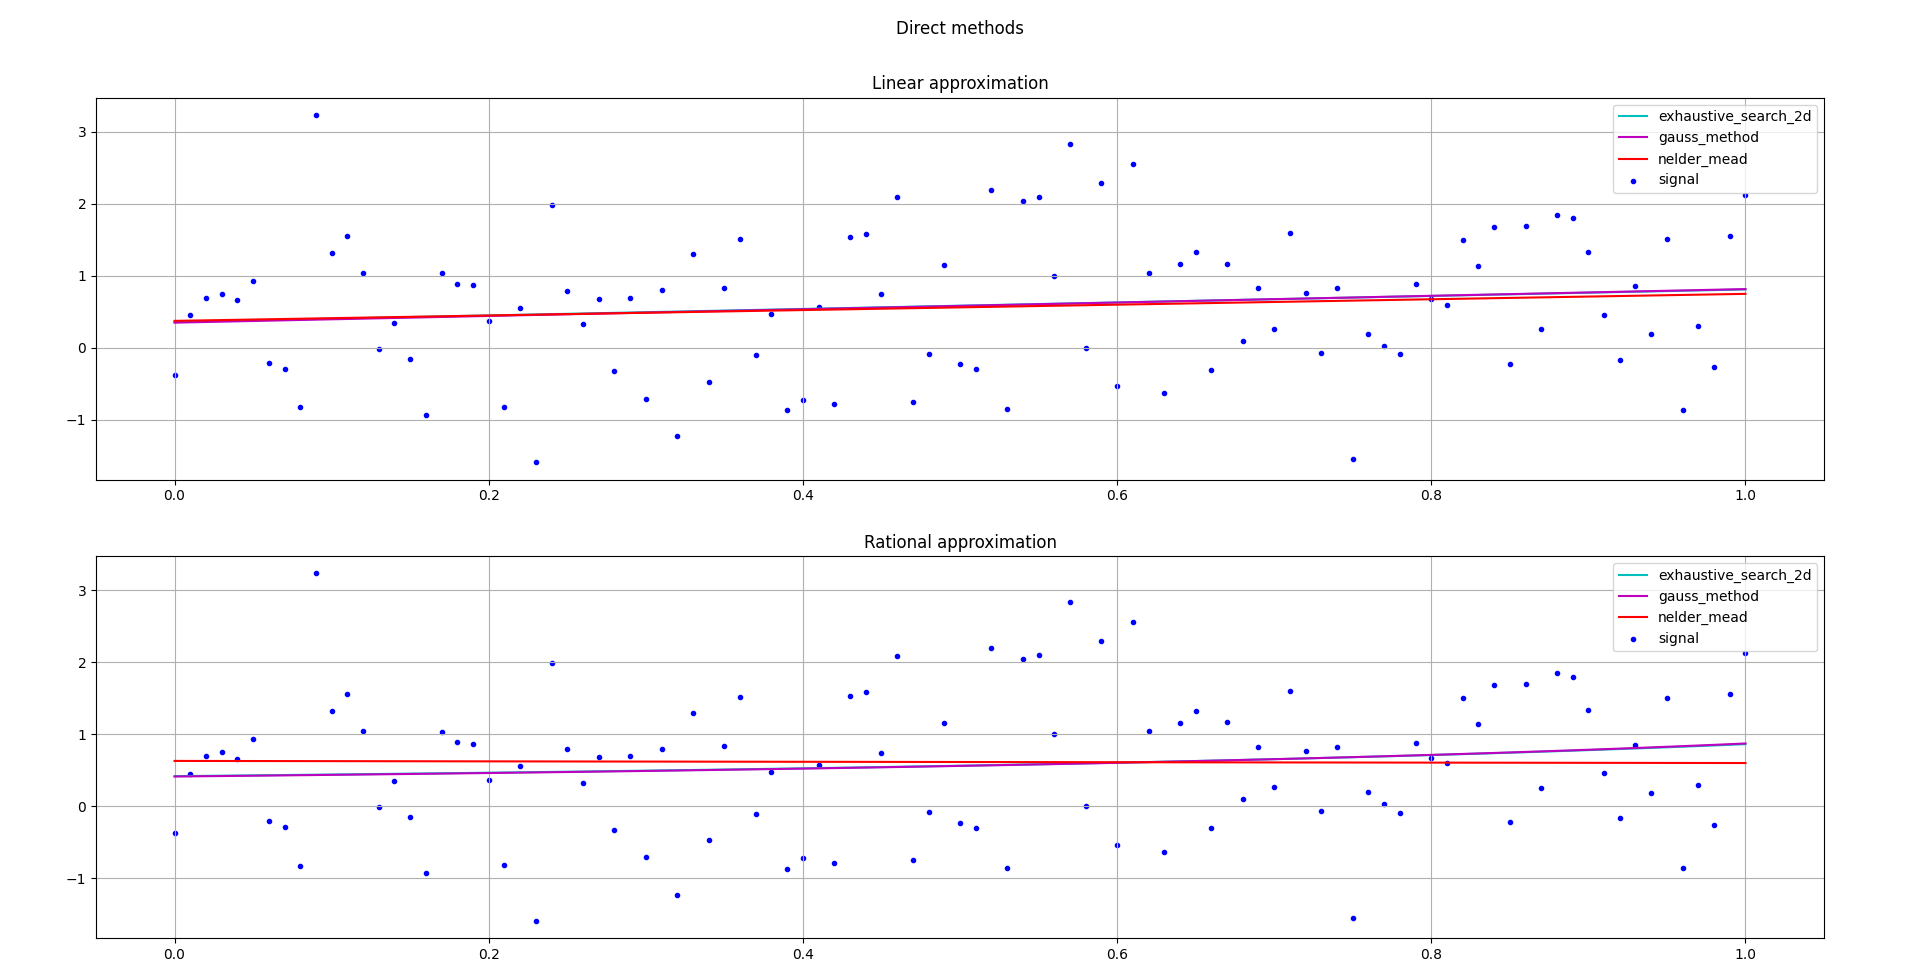
\includegraphics[width=\textwidth]{img/plot.png}
    \caption{Direct methods of optimization.}
    \label{ris:direct}
\end{figure}

\subsection{Conclusion}

In the course of the laboratory work, direct methods were implemented and analyzed within the problem of the unconstrained optimization problem.

\subsection{Appendix}

The source code is located \href{https://github.com/vanSultan/anal_dev_algo/tree/lab_02}{here}: \url{https://github.com/vanSultan/anal_dev_algo/tree/lab_02}.
